% Gemini theme
% https://github.com/anishathalye/gemini

\documentclass[final]{beamer}

% ====================
% Packages
% ====================

\usepackage[T1]{fontenc}
\usepackage{lmodern}
% \usepackage[size=custom,width=120,height=72,scale=1.0]{beamerposter}
\usepackage[size=a0,orientation=landscape,scale=1.0]{beamerposter}
\usetheme{gemini}
\usecolortheme{bristol}
\usepackage{graphicx}
\usepackage{booktabs}
\usepackage{tikz}
\usepackage{pgfplots}
\pgfplotsset{compat=1.14}
\usepackage{anyfontsize}

\usepackage{minted}
\setminted[python]{
    linenos,
    % bgcolor=LightGray,
    % breaklines,
    fontsize=\scriptsize,
    % xleftmargin=1.1em,
    numbersep=4pt
}

\usepackage{tcolorbox}

\newtcolorbox[auto counter]{pbox}[2][]{
  colback=white,
  title=#2,
  #1,
  fonttitle= \large, %\sffamily,
  % fontupper=\sffamily,
  boxrule=0.5pt, 
  arc=2pt,
  top=1pt, 
  bottom=1pt,
  before={\vspace{2pt}}, 
  after={\vspace{2pt}} 
  % colframe=..,
  % coltitle=..,
  % colbacktitle=..,
  % toptitle=0.05cm,
  % bottomtitle=0.125cm
}

\usepackage{fancyvrb}

% ====================
% Lengths
% ====================

% If you have N columns, choose \sepwidth and \colwidth such that
% (N+1)*\sepwidth + N*\colwidth = \paperwidth
\newlength{\sepwidth}
\newlength{\colwidth}
\setlength{\sepwidth}{0.025\paperwidth}
\setlength{\colwidth}{0.3\paperwidth}

\newcommand{\separatorcolumn}{\begin{column}{\sepwidth}\end{column}}

% ====================
% Title
% ====================

\title{Position: Don't Use the CLT in LLM Evals With Fewer \\ \vspace{1cm} Than a Few Hundred Datapoints \quad \huge{(...it's \textit{really} easy to do \textit{a lot} better!)}}

\author{\;Sam Bowyer \inst{1} \and Laurence Aitchison \inst{1, \star} \and Desi R. Ivanova \inst{2,\star}}

\institute[shortinst]{\inst{1} University of Bristol \samelineand \inst{2} University of Oxford \samelineand \inst{\star} Equal Contribution\vspace{1cm}}

% ====================
% Footer (optional)
% ====================

\footercontent{
  \href{https://github.com/sambowyer/bayes_evals}{github.com/sambowyer/bayes\_evals} \hfill
  ICML 2025 Spotlight Position Paper \hfill
  \href{mailto:sam.bowyer@bristol.ac.uk}{sam.bowyer@bristol.ac.uk}}
% (can be left out to remove footer)

% ====================
% Logo (optional)
% ====================

% use this to include logos on the left and/or right side of the header:
% \logoright{\includegraphics[height=7cm]{logo1.pdf}}
% \logoleft{\includegraphics[height=7cm]{logo2.pdf}}

% ====================
% Body
% ====================

\begin{document}

% \addtobeamertemplate{headline}{} 
% {
%     \begin{tikzpicture}[remember picture,overlay] 
%     \node [anchor=north east, inner sep=1cm] at ([xshift=-3cm,yshift=0cm]current page.north east) {
%         % \includegraphics[height=15cm]{fig/logos/UoB_logo_White_24.pdf}
%         \includegraphics[height=6cm]{fig/logos/joint3.pdf}
%       }; 
%     \end{tikzpicture} 
% }
% \logoright{\includegraphics[height=15cm]{fig/logos/UoB_logo_White_24.pdf}}
% \logoright{
%   % \begin{center}
%     % 
\includegraphics[height=15cm]{fig/logos/oxford.png}
%     % \\
%     % \vspace{-1cm}
%     % \includegraphics[height=13cm]{fig/logos/UoB_logo_White_24.pdf}
%     % \vspace{-0.5cm}
%   % \end{center}
%   % \includegraphics[height=13cm,clip=true,trim=2cm 2cm 2cm 2cm]{fig/logos/combined_logo.pdf}
%   % \vspace{1.5cm}
%   % \includegraphics[height=10cm]{fig/logos/combined_logo.pdf}
%   \includegraphics[height=6cm]{fig/logos/joint3.pdf}
%   \vspace{2cm}
% }

\begin{frame}[fragile]
\begin{columns}[t]
\separatorcolumn

\begin{column}{\colwidth}

  \begin{exampleblock}{1. Failures of the Central Limit Theorem}

    % \begin{theorem}{Central Limit Theorem}
    \textbf{Central Limit Theorem:}
    If $X_1, \ldots, X_N$ are IID r.v.s with mean $\mu \in \mathbb{R}$ and finite variance $\sigma^2$, then with sample mean $\hat{\mu} = \frac{1}{N}\sum_{i=1}^N X_i$,
    $$\sqrt{N} (\hat{\mu} - \mu) \xrightarrow{d} \mathcal{N} \left( 0, \sigma^2 \right) \; \text{as } N \rightarrow \infty.$$
    % \end{theorem}

    % horizontal line
    \begin{center}
      \rule{0.8\textwidth}{0.4pt}
    \end{center}

    % \textbf{CLT-based confidence interval} on binary data $y_i \in \{0, 1\}$ (incorrect/correct) for $i=1,\ldots,N$, with standard error $\sqrt{\bar{y}(1-\bar{y})/N}$:
    \textbf{CLT-based confidence interval} on binary data 
    $$ y_i = \begin{cases} 0 & \text{question } i \text{ answered incorrectly} \\ 1 & \text{question } i \text{ answered correctly} \end{cases} $$
    for $i=1,\ldots,N$, with standard error $SE(\bar{y}) = \sqrt{\bar{y}(1-\bar{y})/N}$:
    $$
    \text{CI}_{1-\alpha} = \bar{y} \pm z_{\alpha/2} \text{SE}(\bar{y}),
    $$
    where $z_{\alpha/2}$ is the $(\alpha/2)$-th quantile of $\mathcal{N}(0, 1)$, e.g. $z_{0.025} = 1.96$.% for $95\%$ CI.
    % \\
    % That is, we model the true probability of success $\theta$ as $\mathcal{N}(\bar{y}, \text{SE}(\bar{y}))$.

    \begin{figure}
      \centering
      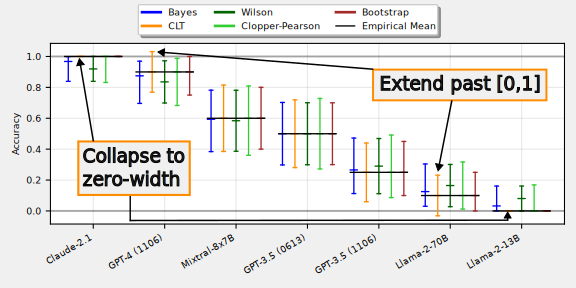
\includegraphics[width=0.95\textwidth]{fig/PLOTS_FINAL_GREY/pdfs/real_data_langchain_poster_plot.pdf}
      % \caption{Langchain Typewriter tool-use benchmark ($N=20$).}
    \end{figure}

    % As LLM capabilities improve, it's becoming more common to run small-$N$ benchmarks, for which CLT-based error bars can \textbf{collapse to zero-width} or \textbf{extend past [0,1]}.
    As LLM capabilities improve, it's becoming more common to run small-$N$ benchmarks, e.g. the Langchain Typewriter tool-use benchmark shown above ($N=20$).
    
  \end{exampleblock}

  \begin{exampleblock}{2. Simulation Setup}

    \begin{enumerate}
      \item \textbf{Synthetic datasets}: Draw probability of success 
      $$\theta \sim \text{Uniform}[0, 1],$$
      then draw $N$ IID samples 
      $y_i \sim \text{Bernoulli}(\theta).$%, i=1,\ldots,N$.
      \item \textbf{Construct intervals with various confidence levels} 
      $$1-\alpha \in [0.8, 0.995].$$
      % \item Repeat.
      \item \textbf{Repeat} the above many times, and compare different interval-construction methods via
        \begin{itemize}
          \Large
          \item \textbf{Coverage} (proportion of intervals that contain true value of $\theta$; should equal $1-\alpha$)
          \item \textbf{Interval width}
        \end{itemize}
    \end{enumerate}

    % Repeat the above and compare different interval-construction methods via \textbf{coverage} (proportion of intervals that contain true value of $\theta$; should equal $1-\alpha$) and \textbf{interval width}.

    % \begin{figure}
    %   \centering
    %   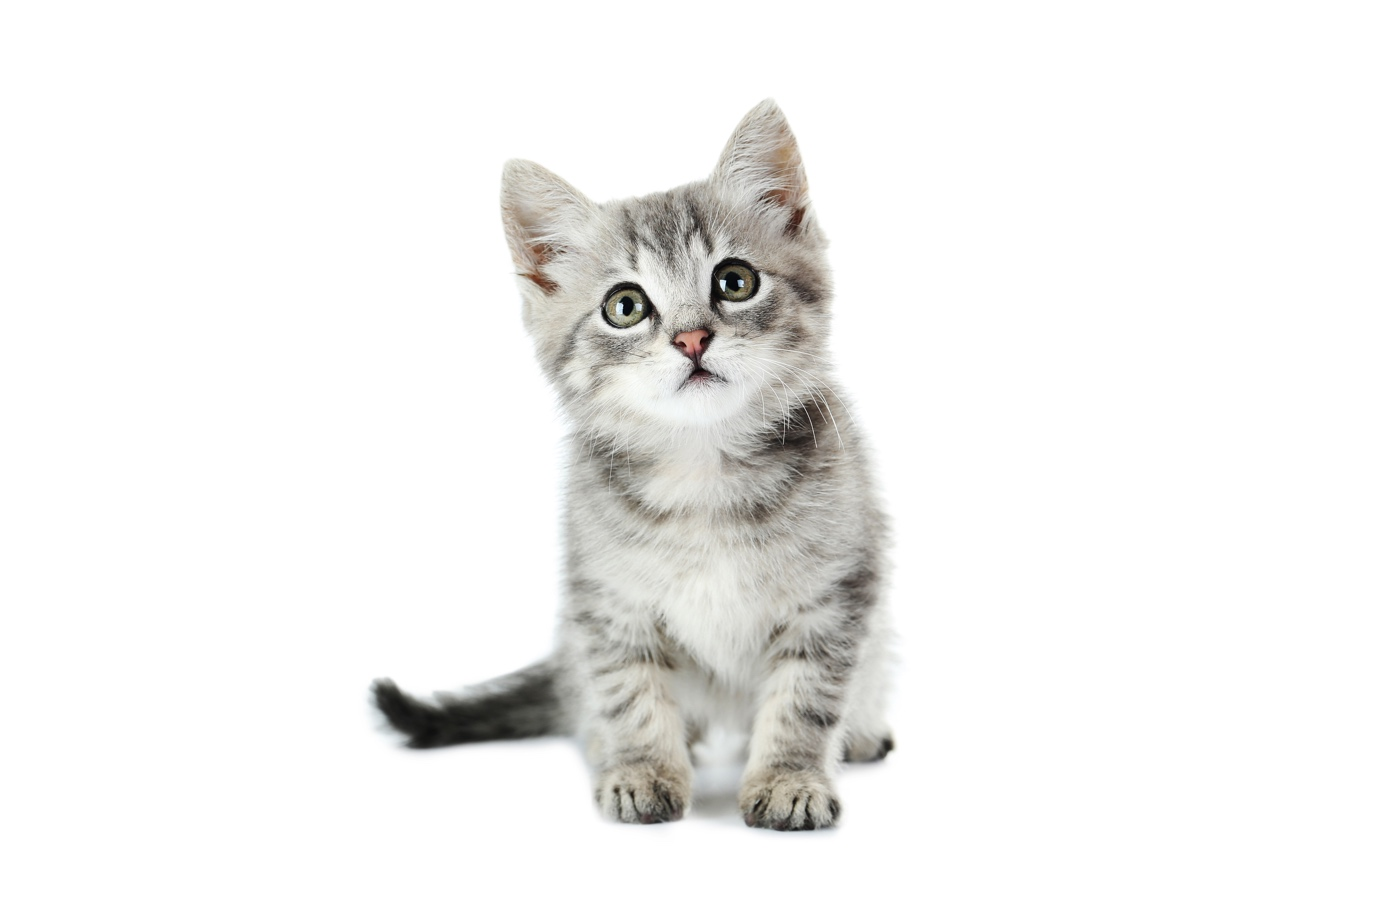
\includegraphics[width=0.75\textwidth]{fig/kitten.jpg}
    % \begin{figure}


  \end{exampleblock}

\end{column}

\separatorcolumn

\begin{column}{\colwidth}

  \begin{block}{3. Alternative Interval Construction}

    \textbf{Bayesian Beta-Bernoulli credible interval} --- uniform prior over probability of success $\theta$:
    $$
    \begin{aligned}
      \theta &\sim \text{Beta}(1, 1) = \text{Uniform}[0, 1] \\
      y_i &\sim \text{Bernoulli}(\theta) \; \text{for } i=1,\dots N 
    \end{aligned}
    $$
    Use quantiles of closed-form posterior to construct $1-\alpha$ CIs:
    $$
    \theta \mid y_{1:N} \sim \text{Beta}\left(1 + \sum_{i=1}^N y_i, 1 + N - \sum_{i=1}^N y_i\right)
    $$

    % code
    \begin{pbox}[label={ex:bayes_simple}]{Beta-Bernoulli Bayesian Credible Interval}
    \begin{minted}[fontsize=\large,breaklines]{python}
posterior = scipy.stats.beta(1 + sum(y), 1 + N - sum(y))
bayes_ci  = posterior.interval(confidence=0.95)
    \end{minted}
    \end{pbox}

    \vspace{-1.25em}
    % horizontal line
    \begin{center}
      \rule{0.8\textwidth}{0.4pt}
    \end{center}

    \textbf{Wilson Score confidence interval} --- based on binomial distribution:
    $$
    \text{CI}_{1-\alpha, \text{Wilson}} = \frac{\hat{\theta} + \frac{z_{\alpha/2}^2}{2N}}{1 + \frac{z_{\alpha/2}^2}{N}} \pm \frac{\frac{z_{\alpha/2}}{2N}}{1 + \frac{z_{\alpha/2}^2}{N}}\sqrt{4N\hat{\theta}(1 - \hat{\theta}) + z_{\alpha/2}^2}.
    $$
    % where $z_{\alpha/2}$ is the $(1-\alpha/2)$-th quantile of $\mathcal{N}(0, 1)$. 

    % code
    \begin{pbox}[label={ex:wilson_simple}]{Wilson Score Confidence Interval}
    \begin{minted}[fontsize=\large,breaklines]{python}
result = scipy.stats.binomtest(k=sum(y), n=N)
wilson_ci = result.proportion_ci("wilson", 0.95)
    \end{minted}
    \end{pbox}

    \vspace{-1.25em}
    % horizontal line
    \begin{center}
      \rule{0.8\textwidth}{0.4pt}
    \end{center}

    \textbf{Clopper-Pearson confidence interval} --- `exact' method based on cumulative binomial distribution.
    Contains all values $\theta_0$ that won't reject a two-sided test with null $H_0: \theta = \theta_0$ at significance level $\alpha$.
    % Includes all values of $\theta_0$ that are \textit{not} possible to reject at the $1-\alpha$ level with the null hypothesis $H_0: \theta = \theta_0$.

    % code
    \begin{pbox}[label={ex:clopper_simple}]{Clopper-Pearson Confidence Interval}
      \begin{minted}[fontsize=\large,breaklines]{python}
  result = scipy.stats.binomtest(k=sum(y), n=N)
  clop_ci = result.proportion_ci("exact", 0.95)
      \end{minted}
      \end{pbox}

    % % horizontal line
    % \begin{center}
    %   \rule{0.8\textwidth}{0.4pt}
    % \end{center}

    % \textbf{Bootstrap}: quantile-based interval on $\hat{\theta} = \bar{y}$ from resampled data.
  
  \end{block}

  \vspace{-1em}

  \begin{block}{4. Results}

    \begin{figure}
      \centering
      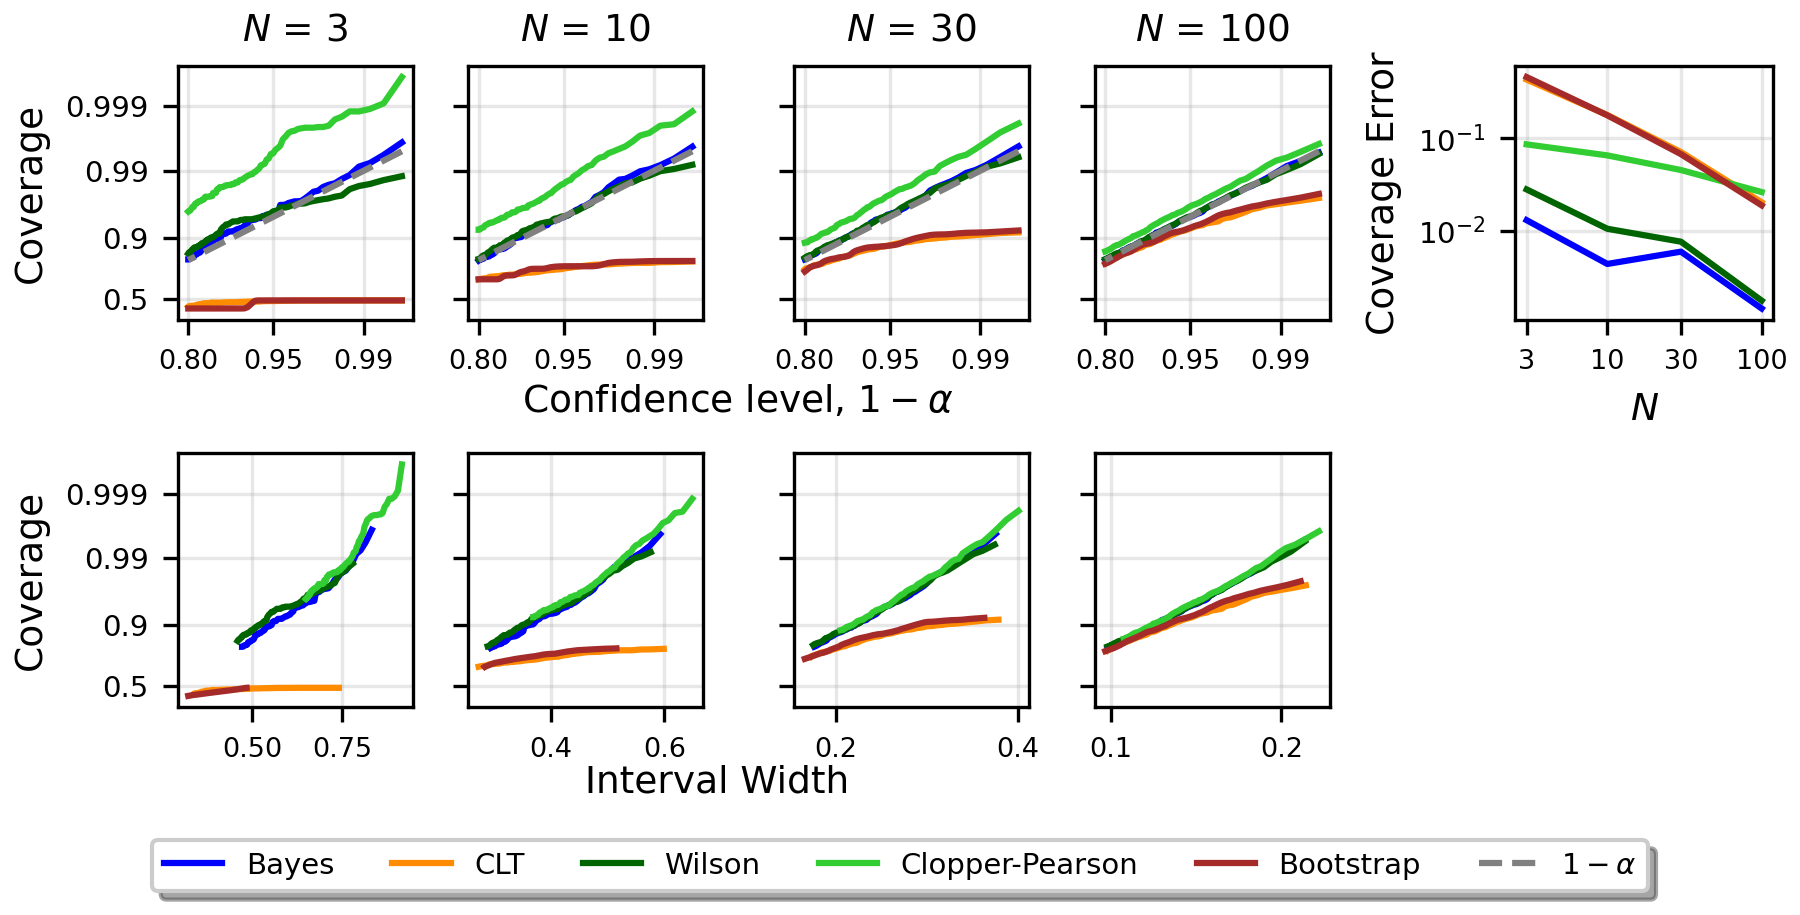
\includegraphics[width=\textwidth]{fig/pdfs/exp4-1.pdf}
      % \caption{}
    \end{figure}

  \end{block}

\end{column}

\separatorcolumn

\begin{column}{\colwidth}

  \begin{exampleblock}{5. Other Settings}

    \begin{itemize}
      \item \textbf{Mismatched Prior} --- Different prior for data simulation e.g. 
      $\theta \sim \text{Beta}(100,20), \quad \mathbb{E}[\theta] = 0.83, \quad \text{Var}[\theta] = 0.034^2.$ \\
      % \vspace{-1em}
      \begin{figure}
        \centering
        \includegraphics[width=0.9\textwidth]{fig/PLOTS_FINAL_GREY/pdfs/exp4-1_beta-100-20_mismatch_alpha_only.pdf}
        % \vspace{-1em}
        % \caption{\textbf{Clustered questions setting}: with $N_t = 5$ questions per task.}
      \end{figure}
      % \vspace{-0.5em}
      \item \textbf{Clustered Questions} --- $T$ tasks, each with $N_t$ IID questions.
      Clustered CLT uses a different standard error formulation:
      $$
      \text{SE}_\text{clust.} = \sqrt{\text{SE}_\text{CLT}^2 + \frac{1}{N^2}\sum_{t=1}^T \sum_{i=1}^{N_t} \sum_{j \neq i} (y_{i,t} - \bar{y})(y_{j,t} - \bar{y})}.
      % \text{SE}_\text{clust.} = \sqrt{\text{SE}_\text{CLT}^2 + (1/N^2)\sum_{t=1}^T \sum_{i=1}^{N_t} \sum_{j \neq i} (y_{i,t} - \bar{y})(y_{j,t} - \bar{y})}.
      $$
      Bayesian credible interval found via importance sampling:
      $$
        \begin{aligned}
        \theta &\sim \text{Beta}(1, 1), \quad 
        &&d \sim \text{Gamma}(1, 1), \quad \\
        \theta_t &\sim \text{Beta}(d \theta, d (1-\theta)), \quad
        &&y_{i,t} \sim \text{Bernoulli}(\theta_t).
        \end{aligned}
      $$
      
      \begin{figure}
        \centering
        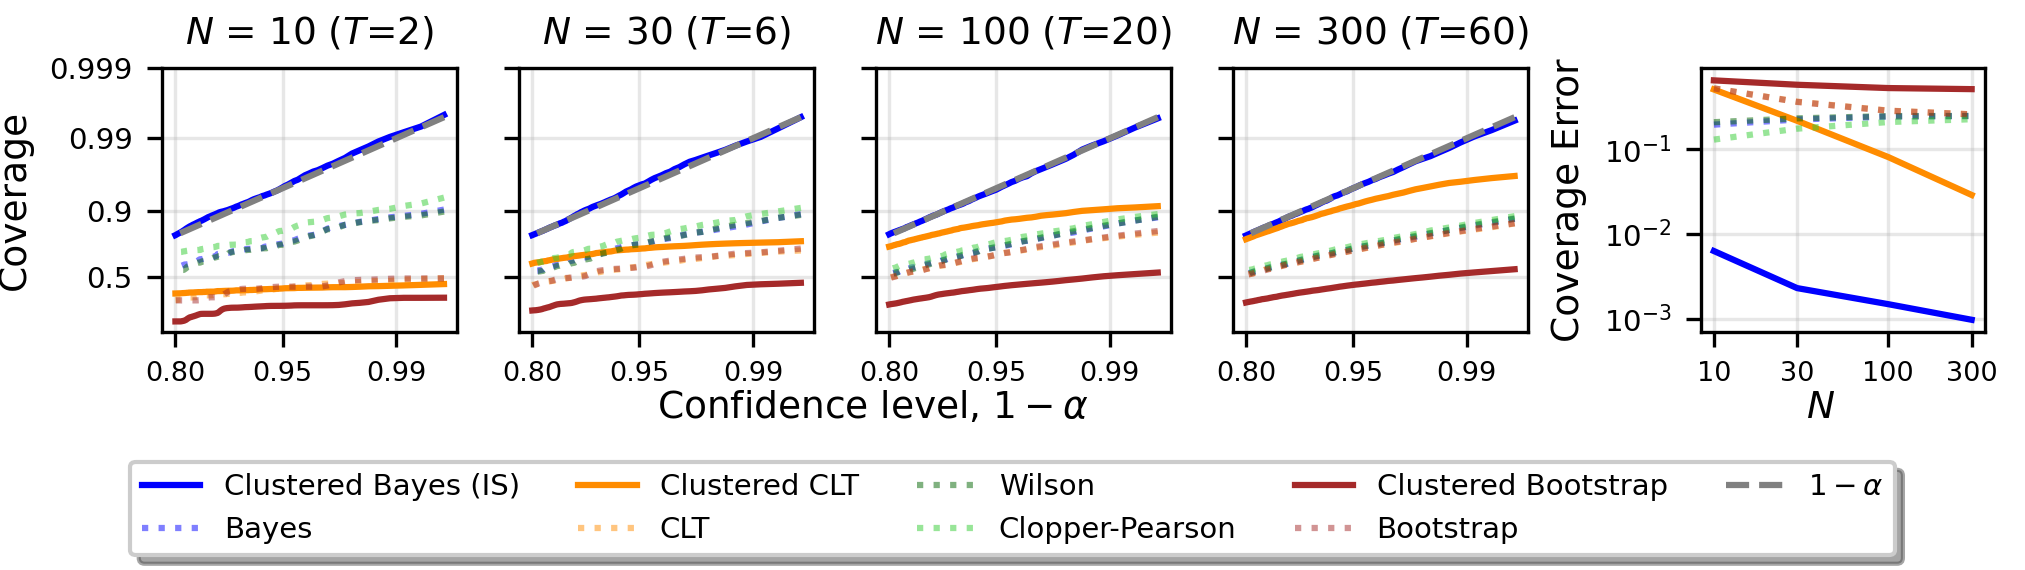
\includegraphics[width=0.9\textwidth]{fig/PLOTS_FINAL_GREY/pdfs/exp4-2_alpha_only.pdf}
        % \vspace{-1em}
        % \caption{\textbf{Clustered questions setting}: with $N_t = 5$ questions per task.}
      \end{figure}
      \item \textbf{Independent Comparisons} --- Compare $\theta_A$ and $\theta_B$ for two different models, with access \textit{only} to $N_A, N_B, \bar{y}_A,$ and $\bar{y}_B$.
      \item \textbf{Paired Comparisons} --- Compare $\theta_A$ and $\theta_B$ for two different models, each with the same $N$ IID questions and access to question-level successes $\{y_{A;i}\}_{i=1}^N$ and $\{y_{B;i}\}_{i=1}^N$.
      \item \textbf{Metrics that aren't simple averages} --- e.g. F1 score.
    \end{itemize}

    We construct Bayesian credible intervals that outperform CLT-based intervals in all settings (available in \textbf{\texttt{bayes\_evals}}).

  \end{exampleblock}


  \vspace{-0.75em}
  \begin{alertblock}{6. Recommendations}
    
    % two-column of figures
    \begin{columns}
      \begin{column}{0.7\textwidth}
        % \vspace{-1.5em}

        \begin{itemize}
          \item \textbf{IID setting:} use \textbf{Beta-Bernoulli} credible intervals or \textbf{Wilson score} confidence intervals via \textbf{\texttt{scipy}} or equivalent.
          
          \item \textbf{Other settings:} use \textbf{Bayesian credible intervals} as implemented in our simple package \textbf{\texttt{bayes\_evals}}.
        \end{itemize}
        % \vspace{-0.5em}
      \end{column}
      \begin{column}{0.3\textwidth}
        \vspace{1em}
        \begin{figure}
          \centering
          
\includegraphics[width=0.5\textwidth]{fig/arxiv_qr.png}
          % \caption{}
        \end{figure}

        \vspace{0.5em}
      
        \begin{figure}
          \centering
          
\includegraphics[width=0.5\textwidth]{fig/github_qr.png}
          % \caption{}
        \end{figure}
      \end{column}
    \end{columns}

  \end{alertblock}

  % \begin{block}{References}

  %   \nocite{*}
  %   \footnotesize{\bibliographystyle{plain}\bibliography{poster}}

  % \end{block}

\end{column}

\separatorcolumn
\end{columns}

\begin{tikzpicture}[remember picture,overlay] 
  \node [anchor=north east, inner sep=1cm] at ([xshift=-2.75,yshift=-2.5cm]current page.north east) {
      \includegraphics[height=5.25cm]{fig/logos/joint3.pdf}
    }; 
\end{tikzpicture} 

\end{frame}

\end{document}
